\documentclass[tikz,border=8pt]{standalone}
% Shared look for every TikZ diagram. Load with \input{../../tools/tikz-style.tex}
\usepackage[T1]{fontenc}
\usepackage{lmodern}
\renewcommand{\sfdefault}{lmr}  % diagrams use the same serif as the text
\usetikzlibrary{arrows.meta, positioning, shapes.geometric, calc, fit, backgrounds}
\definecolor{cblue}{HTML}{4C78A8}
\definecolor{corange}{HTML}{F58518}
\definecolor{cgreen}{HTML}{54A24B}
\definecolor{cred}{HTML}{E45756}
\definecolor{cpurple}{HTML}{B279A2}
\definecolor{cgrey}{HTML}{6B6B6B}
\tikzset{
  every picture/.style={font=\sffamily, line width=1.2pt},
  box/.style={draw=#1, fill=#1!12, rounded corners=4pt, align=center, inner sep=7pt, minimum height=1.1cm},
  box/.default=cgrey,
  arrow/.style={-{Stealth[length=3mm]}, draw=cgrey, line width=1.4pt},
  title/.style={font=\sffamily\bfseries\Large},
  note/.style={font=\sffamily\small, text=cgrey, align=center},
}
\AtBeginDocument{\hyphenpenalty=10000 \exhyphenpenalty=10000}

\newcommand{\col}[4]{% x, header, colour, list of cells
  \node[box=#3, minimum width=2.6cm, minimum height=0.8cm, inner sep=3pt, font=\sffamily\bfseries] at (#1,0) {#2};
  \foreach \v [count=\i] in {#4}
    \node[draw=#3, fill=white, minimum width=2.6cm, minimum height=0.75cm] at (#1,-0.78*\i) {\v};
}
\begin{document}
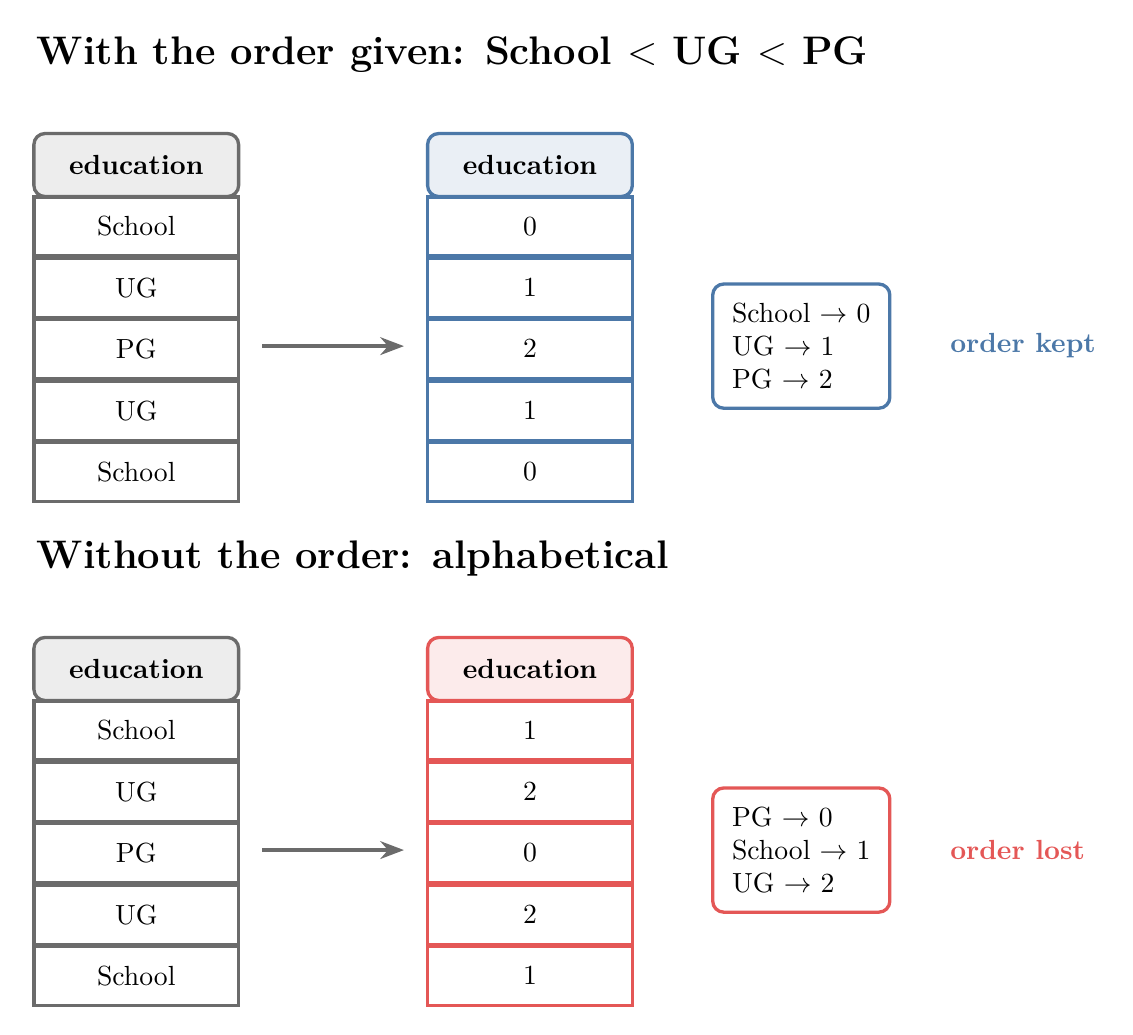
\begin{tikzpicture}
  % top: order given
  \node[title, anchor=west] at (-1.4,1.4) {With the order given: School $<$ UG $<$ PG};
  \col{0}{education}{cgrey}{School,UG,PG,UG,School}
  \draw[arrow] (1.6,-2.3) -- (3.4,-2.3);
  \col{5}{education}{cblue}{0,1,2,1,0}
  \node[box=cblue, fill=white, align=left, anchor=west] at (7.3,-2.3) {School $\rightarrow$ 0\\ UG $\rightarrow$ 1\\ PG $\rightarrow$ 2};
  \node[font=\sffamily\bfseries, text=cblue, anchor=west] at (10.2,-2.3) {order kept};
  % bottom: default
  \begin{scope}[yshift=-6.4cm]
  \node[title, anchor=west] at (-1.4,1.4) {Without the order: alphabetical};
  \col{0}{education}{cgrey}{School,UG,PG,UG,School}
  \draw[arrow] (1.6,-2.3) -- (3.4,-2.3);
  \col{5}{education}{cred}{1,2,0,2,1}
  \node[box=cred, fill=white, align=left, anchor=west] at (7.3,-2.3) {PG $\rightarrow$ 0\\ School $\rightarrow$ 1\\ UG $\rightarrow$ 2};
  \node[font=\sffamily\bfseries, text=cred, anchor=west] at (10.2,-2.3) {order lost};
  \end{scope}
\end{tikzpicture}
\end{document}
